%File: submission.tex --- AAAI-27 anonymous submission
% "An Empirical Analysis of Transfer for Dynamic Path Planning"
% Built on the official AAAI-27 author kit (aaai2027.sty, TemplateVersion 2027.1).
\documentclass[letterpaper]{article} % DO NOT CHANGE THIS
\usepackage[submission]{aaai2027}  % DO NOT CHANGE THIS
\usepackage[hyphens]{url}  % DO NOT CHANGE THIS
\usepackage{graphicx} % DO NOT CHANGE THIS
\urlstyle{rm} % DO NOT CHANGE THIS
\def\UrlFont{\rm}  % DO NOT CHANGE THIS
\usepackage{natbib}  % DO NOT CHANGE THIS AND DO NOT ADD ANY OPTIONS TO IT
\usepackage{caption} % DO NOT CHANGE THIS AND DO NOT ADD ANY OPTIONS TO IT
\frenchspacing  % DO NOT CHANGE THIS
%
% Recommended for better-looking tables
\usepackage{booktabs}
\usepackage{amsmath}
%
\pdfinfo{
/TemplateVersion (2027.1)
}
\setcounter{secnumdepth}{0}

% Custom macros
\newcommand{\stage}[1]{\textsc{#1}}

\title{An Empirical Analysis of Transfer for Dynamic Path Planning}
\author{
    Anonymous Submission
}
\affiliations{
}

\begin{document}

\maketitle

\begin{abstract}
We study the dynamic path planning problem, where an agent needs to plan a route in the presence of moving obstacles. This problem is relevant for all agents that need to navigate in the real world. In particular, we study whether heuristics learned in training maps can be transferred---zero-shot or from a few labeled target maps---to new environments for this task. We show that, with the right training objective and planner integration, heuristics transfer zero-shot in both discrete and continuous environments---even heuristics given no information about future obstacle motion---matching or improving success in new maps while substantially reducing search effort. With a few labeled target maps, low-rank adaptation preserves the transferred prior while full fine-tuning overtakes it as labels accumulate---and a single dynamic map is already label-rich. Further, this is agnostic to model architecture choices in that Multilayer Perceptrons, Long Short-Term Memory models, Hierarchical Reasoning Models and U-Net architectures of comparable complexity all can be used with similar success rates.
\end{abstract}

% Uncomment the following to link to your code, datasets, an extended version or similar.
% You must keep this block between (not within) the abstract and the main body of the paper.
% Make sure that you do not de-anonymize yourself with these links.
% \begin{links}
%     \link{Code}{https://anonymous.4open.science/}
% \end{links}

\section{Introduction}

An agent navigating the real world rarely plans on an empty, static map: pedestrians cross corridors, vehicles occupy lanes, doors open and close. Planning a route in the presence of moving obstacles---the \emph{dynamic path planning} problem---is correspondingly harder than its static counterpart, because the search must reason over space \emph{and} time \citep{silver2005cooperative,phillips2011sipp}, and the simple admissible heuristics that make A\textsuperscript{*} \citep{hart1968astar} efficient on static maps become badly uninformed once waiting, detouring, and timing matter. Learned heuristics promise to close this gap \citep{arfaee2011bootstrap,bhardwaj2017sail,yonetani2021neuralastar}, but they only help a deployed agent if they work in environments the agent has never seen: a heuristic that must be retrained on the deployment map defeats its own purpose. This paper therefore asks an empirical question with direct practical stakes: \emph{do heuristics learned on training maps transfer---zero-shot, or from a few labeled target maps---to new environments for dynamic path planning?}

Answering this question fairly is harder than it looks, because transfer results are routinely confounded by factors that have nothing to do with transfer: the objective the heuristic was trained on, the way its output enters the planner, and the amount of supervision a ``shot'' actually contains. Our study therefore pairs every claim with controls that isolate these factors---twin models differing in exactly one input, integration comparisons that reuse identical frozen weights, calibrated benchmarks on which the classical baseline is neither saturated nor hopeless, preregistered evaluation gates with hard stops, and paired statistics clustered at the map level \citep{henderson2018matters,agarwal2021precipice,pineau2021reproducibility}. We use static suites deliberately as a \emph{proving ground}: labels there are exact and confounds controllable, so harness choices can be validated before being cashed in on the dynamic target, where the baseline is weakest and learned guidance matters most.

Across a discrete grid-world program and a continuous roadmap program \citep{kavraki1996prm} spanning thirteen preregistered stages, we find:
\begin{itemize}
    \item \textbf{Zero-shot transfer works in both spaces---once the harness is right.} On calibrated continuous benchmarks, transferred heuristics raise success by up to $+0.475$ on unseen static maps and $+0.2$ to $+0.7$ on unseen dynamic maps while cutting matched search effort by 15--48\% (static) and 62--95\% (dynamic). On discrete grids, the \emph{same frozen weights} that are useless as an additive correction to a tight Manhattan baseline deliver a 6--15\% reduction, with no observed loss of success, when used to \emph{rank} within an admissible band---transfer was never the obstacle; integration was.
    \item \textbf{No future-motion information is needed.} Twin heuristics differing only in an 8-step future obstacle window show no systematic accuracy or search advantage for the future-aware twin, and few-shot adaptation does not unlock one (no significant cell in nine, map-clustered). Present-frame heuristics suffice for the dynamic benchmarks we test.
    \item \textbf{Few-shot adaptation splits into two supervision regimes.} Rank-8 low-rank adapters preserve the transferred prior when labels are scarce, while full fine-tuning is unstable early and overtakes them once labels accumulate (map-clustered crossover with disjoint confidence intervals). The regime variable is supervision density, not map count: a single dynamic map already supplies roughly 25{,}000 labeled space--time states, dissolving the scarce regime entirely.
    \item \textbf{Architecture is largely a free choice---the harness is not.} Under a matched harness, Multilayer Perceptrons, LSTMs, Hierarchical Reasoning Models, and U-Nets of comparable complexity reach similar success. Architectural hierarchy specifically never converts added depth into growing advantage on deeper problems---learned halting even \emph{anti-}correlates with problem depth---and our strongest single result is an architecture-minimal one: a small MLP restricted to bounded local observations, integrated with one inference-time Bellman backup, beats every complete-map provider we trained, including the strongest hierarchical one, by 15.95\% pooled expansions at matched empirical path quality on 144 held-out maps.
\end{itemize}

Figure~\ref{fig:map} maps the experimental program onto the three harness ingredients our analysis isolates; Table~\ref{tab:matrix} summarizes every stage and verdict at the strength its evidence supports.

\begin{table*}[t]
\centering
\footnotesize
\begin{tabular}{@{}p{1.5cm}p{3.3cm}p{3.6cm}p{8.0cm}@{}}
\toprule
Stage & Protocol & Question & Verdict (headline evidence) \\
\midrule
\stage{C1--C4} & easy roadmap pilots & do learned bases/experts help? & saturated; Euclid 0.925--1.00 success; specialists $\leq$3\% \\
\stage{C5} & calibrated hard maps, scalar & learned scalar guidance? & ON-LSTM $+0.48$ succ.\ ($q{=}4{\times}10^{-11}$); HRM collapses to cap \\
\stage{C6} & value-field objective & does the objective rescue HRM? & yes: 0.625$\to$0.975 succ.\ ($q{=}3.4{\times}10^{-4}$) \\
\stage{C7} & static integration matrix & additive vs.\ focal vs.\ scalar/field & additive wins vs.\ loose Euclid; ratios 0.43--0.85; subopt.\ 1.02--1.14 \\
\stage{C8} & space--time dynamics, twins & dynamic transfer? future window? & ratios 0.046--0.380; no systematic aware benefit (7 blind vs.\ 1 aware) \\
\stage{Discrete} & grids, Manhattan baseline & additive vs.\ focal ranking & additive inert/harmful; same weights focal $w{=}1.0$: $-$6--15\% \\
\stage{C9/C9h} & few-shot static transfer & LoRA vs.\ full FT vs.\ scratch & LoRA preserves at $K{=}1$, plateaus by \emph{capacity} (bound $\Delta{=}0.000{\pm}.008$) \\
\stage{C9b} & few-shot under dynamics & does the crossover persist? & no: $\sim$25k labels/map; 0/9 aware wins; transfer $\gg$ scratch \\
\stage{C10} & zero-label expert interpolation & does composition beat zero-shot? & never better; significantly worse in 2/6 cells despite 0.99 routing \\
\stage{C11} & compositional missions & hierarchy/depth dose--response? & hierarchy gates all negative; halting inverts ($\rho{=}-0.578$ clustered); shallow global-input wins \\
\stage{C12} & hidden regimes; tied refiner & memory? iterative depth? & pilot strongly negative; cycles help monotonically but no $K$ dose--response \\
\stage{C13-A--L} & bounded-observation ladder & what blocks local-observation transfer? & target, then distribution, then \emph{integration}; local backup flips $+16.2\to-1.2$ \\
\stage{C13-M} & frozen 144-map confirmation & does it beat complete-map providers? & yes, all of them: $-12.96$ exp.\ vs.\ field HRM (CI $[-16.3,-9.7]$), matched path quality \\
\stage{C13-N/O/P} & architecture substitution; persistent state & does an HRM (or persistent carry) help? & no: suite-robustness and path-quality gates fail; readout fix transient; persistent carry loses to same-checkpoint reset (MRR $-0.029$) \\
\bottomrule
\end{tabular}
\caption{The experimental program at a glance. Every verdict is stated at the strength its evidence supports (local single-GPU validations; see Limitations). Full per-suite tables, protocols, and statistics appear in the technical appendix.}
\label{tab:matrix}
\end{table*}

\begin{figure*}[t]
\centering

\includegraphics[width=0.98\textwidth]{figures/fig1_program_map.pdf}
\caption{What has to be right for learned heuristics to transfer, and where each stage of the program intervened (orange: failure or negative; blue: positive under the corrected harness; gray: mechanism or null result). Apparent architecture failures were repaired without changing the architecture (\stage{C6} representation rescue; focal ranking; shared-queue certification), while apparent architecture advantages did not survive controls (\stage{C11}, \stage{C12}). The endpoint (\stage{C13-M}) changes only information access and integration and transfers across all six map families.}
\label{fig:map}
\end{figure*}

\section{Problem Setting and Benchmarks}

\textbf{Task.} An agent must reach a goal from a start location on a map containing static obstacles and, in the dynamic setting, obstacles that move along deterministic trajectories. Planning is search-based: A\textsuperscript{*} over a grid (discrete program) or over a probabilistic roadmap \citep[PRM;][]{kavraki1996prm} of $\sim$192 nodes with $k{=}7$ connectivity (continuous program). In dynamic environments the search state is a (location, time) pair, following space--time A\textsuperscript{*} \citep{silver2005cooperative,phillips2011sipp}, so waiting and timing are part of the plan. Every episode carries a per-suite \emph{binding budget} of node expansions, calibrated so that the classical baseline (Manhattan distance on grids; Euclidean distance on roadmaps) is neither saturated nor hopeless; success means reaching the goal within budget.

\textbf{Learned heuristics.} A heuristic provider is trained on a set of \emph{training maps} and queried on maps it has never seen. Supervision is exact where possible: graph-Dijkstra costs-to-go on static roadmaps, and exact backward space--time Dijkstra values over $(\text{node},t)$ states on dynamic ones; the final study replaces these with behavior-derived labels that never read shortest-path values (see Zero-Shot Transfer). Providers span scalar regressors over local features and goal-conditioned raster \emph{value fields} sampled at roadmap nodes, implemented over MLPs, LSTMs \citep{hochreiter1997lstm}, ON-LSTMs \citep{shen2019onlstm}, Hierarchical Reasoning Models \citep[HRM;][]{wang2025hrm} including a faithful port with adaptive computation \citep{graves2016act,banino2021pondernet}, U-Nets \citep{ronneberger2015unet} with FiLM conditioning \citep{perez2018film}, and graph networks; within each comparison, arms are parameter-matched to comparable complexity.

\textbf{Transfer protocol.} We distinguish three transfer distances: unseen maps from the training families; unseen \emph{families} (obstacle statistics never trained on, e.g.\ bugtrap and large-room layouts held out from maze-trained models); and unseen maps under restricted observation (the final study). \emph{Zero-shot} means the provider is applied frozen. \emph{Few-shot} ($K$-shot) means $K$ labeled target maps are available for adaptation, via rank-8 LoRA \citep{hu2021lora}, full fine-tuning, or training from scratch as a control.

\textbf{Metrics and statistics.} We report \emph{success} at the binding budget (paired McNemar tests, Benjamini--Hochberg corrected within families) separately from \emph{matched-solved expansion ratios} (learned over baseline expansions on maps both solve; below 1 is better; bootstrap percentile intervals), and path suboptimality separately again---conditioning on solved maps can otherwise flatter a low-success arm. Because several stages evaluate repeated seeds on the same test maps, inference clusters at the map level: seeds are averaged within maps before any interval or test is computed, and the quantities this paper quotes were recomputed under that grain (10k-resample map-clustered bootstraps; stratified permutation for the halting test). Where a stage's hypothesis needed headroom to be expressible at all, a preregistered oracle gate proved the headroom before any learned arm was trained (e.g., an exact compositional oracle clearing its gate at ratios 0.082--0.225), so null results are informative rather than artifacts of a saturated benchmark. Designs, budgets, and analysis grains were frozen before runs from the seventh stage onward, with hash-bound artifacts and confirmation cohorts generated only after models and integrations were frozen.

\section{Getting the Harness Right}

The abstract's proviso---\emph{with the right training objective and planner integration}---is not a caveat but a finding. Both ingredients, chosen wrongly, produce results that would naturally be misread as transfer or architecture failures; we establish each with a controlled intervention before measuring transfer.

\textbf{Training objective.} On calibrated hard static maps (\stage{C5}), a pooled ON-LSTM regressor trained on scalar cost-to-go residuals transferred superbly to unseen maps (hard-maze success $0.525{\to}1.000$ over Euclid, corrected $q{=}4.3{\times}10^{-11}$), while the identically harnessed HRM \emph{collapsed to a constant} at the label cap and exactly matched the baseline; lower learning rates and a soft cap reproduced the collapse. Changing only the objective---predict a goal-conditioned raster residual \emph{field}, sampled at roadmap nodes (\stage{C6})---rescued the same architecture: HRM success rose $0.625{\to}0.975$ ($q{=}3.4{\times}10^{-4}$). A later stage (\stage{C7}) closed the loop by showing a properly trained scalar model is also viable (ratios 0.427--0.822). The objective, not the architecture and not transfer, determined the outcome in both directions.

\begin{figure}[t]
\centering

\includegraphics[width=0.98\columnwidth]{figures/fig2_integration.pdf}
\caption{The integration inversion. Against a \emph{tight} admissible baseline (discrete grids, Manhattan), additive learned magnitude is inert or harmful (ratios $\geq$1) while the same frozen weights cut expansions 6--15\% as a focal tie-breaker at $w{=}1.0$. Against a \emph{loose} baseline (continuous hard roadmaps, Euclid), additive magnitude wins 15--48\% (field-HRM per-suite ratios shown) and focal variants recover less (range bar).}
\label{fig:integration}
\end{figure}

\textbf{Planner integration.} How the learned estimate enters A\textsuperscript{*} interacts with how tight the classical baseline already is (Figure~\ref{fig:integration}). On continuous hard maps, where Euclidean distance is loose, \emph{additive} learned heuristics dominate: per-suite matched ratios 0.521--0.850 for the field model at path suboptimality only 1.02--1.14, while focal variants \citep{pearl1982semiadmissible,pohl1970} recover less (best post-hoc $w{=}1.1$: 0.789--0.977). On discrete grids the situation inverts. The pooled learned residual there is a near-perfect \emph{ranker} (correlation with the true residual 0.987--0.994 across map sizes) whose \emph{magnitude} is badly scale-flat (predicted/true mean falls from 0.73 to 0.19 as maps grow); injected additively against tight Manhattan it is inert or harmful (in a controlled 22-suite run every learned arm was at or below baseline), yet the same frozen weights used only to rank within the admissible focal band at $w{=}1.0$ cut expansions 6--15\% with no observed success regression---integration-side support for training and consuming heuristics as rankings \citep{chrestien2023rank}. The interaction is causal, not correlational: in a later oracle microcosm, the \emph{exact} value function inserted through a work-discarding two-search integration lost all six test comparisons (141.2 vs.\ 129.7 expansions), and won all six (122.8) when the two searches shared one queue---an integration alone can erase an oracle.

These two results fix the harness for everything that follows: field or properly trained scalar objectives; additive integration on loose baselines, rank-only integration on tight ones.

\section{Zero-Shot Transfer}

We now present the central results, ordered by increasing transfer difficulty.

\textbf{Unseen maps and unseen families (static).} On six calibrated static suites---three training families and three held out entirely---the transferred field model solves 0.75--1.00 of unseen maps against a baseline at 0.25--0.58, with corrected success gains significant on four suites and matched expansion ratios of 0.521--0.850 (\stage{C7}). Family-level transfer is confirmed directly in the adaptation study's zero-shot arms (\stage{C9}): applied frozen to three families never seen in training, pooled providers beat the baseline on success in all six target/backbone cells ($q{=}0.000$--$0.025$).

\textbf{Dynamic environments.} On six dynamic suites with deterministically moving obstacles and exact space--time supervision (\stage{C8}), transferred heuristics take the baseline from success as low as 0.05--0.75 up to 0.75--1.00 on unseen maps ($+0.2$ to $+0.7$; corrected significance on five of six suites) while cutting matched expansions by 62--95\% (ratios 0.046--0.380). This is the paper's headline regime, and it is exactly where the harness analysis predicts learned guidance should pay most: a time-blind Euclidean bound is at its loosest in a moving world, so the additive integration has the most room to help. Path quality is reported separately throughout; the learned arms trade bounded suboptimality (1.02--1.14 on static suites) for these reductions.

\textbf{No future-motion information is needed.} Every dynamic conclusion above holds for heuristics that cannot see obstacle motion at all. We train aware/blind \emph{twins} differing in exactly one input---an 8-step future obstacle window---and find no systematic advantage for awareness: across 24 suite$\times$backbone cells, seven uncorrected significant cells favor the \emph{blind} twin and one favors the aware; direct heuristic accuracy splits 11/24 versus 13/24. Adaptation does not unlock the window either: at full fine-tuning with $K{=}16$ target maps, no cell shows a significant aware advantage (map-clustered deltas $-0.050$ to $+0.017$, all nine intervals crossing zero). We claim no systematic benefit---not harm, and not equivalence---but the practical reading is direct: present-frame heuristics suffice on these benchmarks, so a deployed agent needs no motion predictor in the heuristic loop.

\textbf{Discrete grids, including scale transfer.} On grids the pooled multitask base transfers zero-shot across 22 suites at $+2.11$pp success over Manhattan (descriptive), and the focal-integrated ranker transfers across map \emph{scales} it never trained on, cutting expansions 6--15\% at 128$\times$128 and 192$\times$192 while raising or preserving success (e.g.\ $0.62{\to}0.75$)---the discrete confirmation that the transferable signal was always present and only the integration decides whether it is usable.

\begin{figure*}[t]
\centering
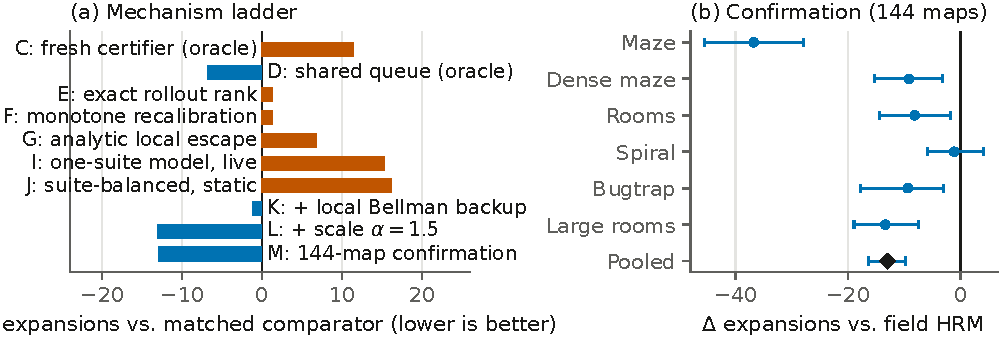
\includegraphics[width=0.98\textwidth]{figures/fig5_c13.pdf}
\caption{Transfer under bounded observation (\stage{C13}). (a) The mechanism ladder: each rung changes one factor; bars are paired expansion deltas versus the matched comparator (rungs C--G versus matched focal search at $w{=}1.10$, including \emph{oracle} providers; rungs I--M versus the preregistered complete-map comparator, a field HRM, live on all six suites). Target and distribution repairs fail; one radius-bounded inference-time Bellman backup (K) plus scale calibration (L) flip the sign. (b) Preregistered confirmation on 144 untouched maps: pooled delta $-12.96$ expansions (95\% CI $[-16.30,-9.74]$; 109 wins/3 ties/32 losses), every suite mean negative, at matched empirical path quality.}
\label{fig:ladder}
\end{figure*}

\textbf{The hardest case: transfer under bounded observation.} Finally, we restrict what the heuristic may see: the estimate for a state must be computed from bounded local observations (a radius-0.20 subgraph) rather than the complete map, and supervision is behavior-derived---median returns of fresh-start local rollouts---never a shortest-path value. This models an agent that cannot assume a global map, and it is deliberately the hardest transfer setting we test. A staged falsification ladder (Figure~\ref{fig:ladder}a) shows what does \emph{not} work: the exact behavior-return statistic itself, replayed with no model error, loses to matched focal search; analytic local-escape constructions are too weak; a model trained on one family fails across the distribution ($+15.4$ expansions, CI $[+12.0,+18.6]$); and suite-balanced retraining \emph{still} fails when inserted statically ($+16.2$). The decisive repair is again integration: a single radius-bounded Bellman backup at inference---kin to one value-iteration step \citep{tamar2016vin} applied at the planner interface---flips the same checkpoint from $+16.2$ to $-1.2$, and scale calibration on fresh maps reaches $-13.0$ (CI $[-18.7,-7.6]$).

Everything was then frozen and 144 zero-overlap confirmation maps were generated across all six families---three of which the model never trained on. The bounded-observation MLP averages 68.31 expansions versus 81.26 for the strongest complete-map provider (a hierarchical field model): paired delta $-12.96$, 95\% CI $[-16.30,-9.74]$, 109/3/32 win/tie/loss, every suite mean negative, with \emph{better} empirical path-cost ratios (mean/max 1.024/1.162 vs.\ 1.031/1.335); it also beats every other complete-map provider we trained (Table~\ref{tab:c13m}). A separate $w{=}1.10$ certified operating point passes all 144 safety checks, cleanly separating the matched-quality direct arm from a formally bounded control. Three caveats travel with this number: one model seed and one confirmation cohort; no formal suboptimality bound on the direct arm; and a prototype feature builder that is slower in wall time than complete-map inference (5.14 s versus 0.37 s per map)---this is a search-effort and path-quality result, not a latency one.

\begin{table}[t]
\centering
\small
\begin{tabular}{lcc}
\toprule
 & Bounded-obs.\ MLP & Field HRM \\
\midrule
Mean expansions $\downarrow$ & \textbf{68.31} & 81.26 \\
Paired $\Delta$ [95\% CI] & \multicolumn{2}{c}{$-12.96$ $[-16.30,\,-9.74]$} \\
Win / tie / loss & \multicolumn{2}{c}{109 / 3 / 32} \\
Suite means negative & \multicolumn{2}{c}{6 / 6} \\
Mean cost ratio $\downarrow$ & \textbf{1.0235} & 1.0311 \\
Max cost ratio $\downarrow$ & \textbf{1.1624} & 1.3346 \\
Valid paths & 144 / 144 & 144 / 144 \\
Feature build (s/map) $\downarrow$ & 5.138 & \textbf{0.371} \\
\bottomrule
\end{tabular}
\caption{Preregistered confirmation of bounded-observation transfer on 144 untouched maps (24 per family; one model seed). Cost ratios are relative to graph-optimal cost. A separate $w{=}1.10$ certified control passes all 144 safety checks. Bold marks the better value.}
\label{tab:c13m}
\end{table}

\section{Few-Shot Adaptation}

\begin{figure}[t]
\centering
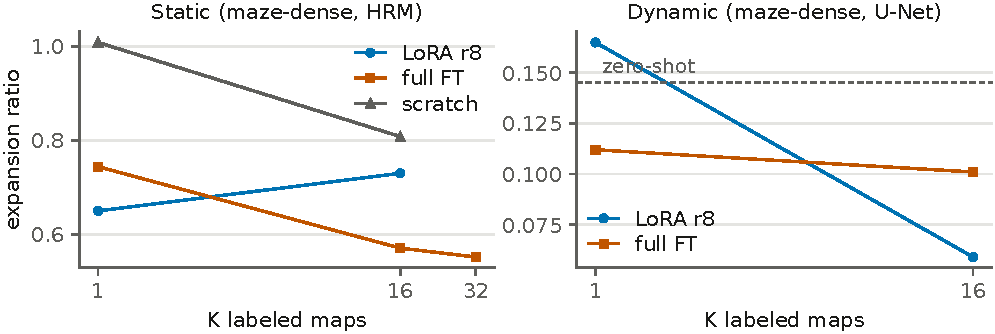
\includegraphics[width=0.98\columnwidth]{figures/fig3_transfer.pdf}
\caption{Supervision density sets the few-shot regime (representative curves; matched-solved ratio vs.\ $K$ labeled target maps, recorded points only). Left: with scarce static labels, rank-8 LoRA preserves the transferred prior at $K{=}1$ while full fine-tuning is unstable early and wins by $K{=}16$--$32$. Right: a single dynamic map already supplies $\sim$25k space--time labels, and the crossover disappears. Points are the canonical record-level curve medians; map-clustered intervals confirm both regimes.}
\label{fig:transfer}
\end{figure}

When a few labeled target maps are available, adaptation behavior is governed by one variable: how much supervision a ``shot'' contains.

\textbf{Scarce labels: preserve the prior.} On static targets, where one map contributes on the order of a few hundred labeled states, rank-8 LoRA at $K{=}1$ preserves the transferred prior essentially intact (maze-dense ratio 0.650 at success 1.00; map-clustered success delta $+0.467$, CI $[+0.300,+0.633]$), while full fine-tuning is high-variance and can be catastrophic (rooms-large $K{=}1$ ratio 1.293, CI $[1.170,1.503]$---worse than the classical baseline); training from scratch is significantly \emph{worse} than the baseline at $K{=}1$ (success delta $-0.167$, CI $[-0.300,-0.047]$). The transferred prior is the asset being protected.

\textbf{Accumulating labels: exploit capacity.} By $K{=}8$--$16$, full fine-tuning overtakes: maze-dense reaches ratio 0.571 and rooms-large 0.500, and at the map-clustered grain the crossover carries disjoint intervals (full fine-tuning 0.610 $[0.549,0.670]$ vs.\ LoRA 0.786 $[0.694,0.891]$ at $K{=}16$). A matched-compute dissection attributes the LoRA plateau precisely: bounded and unbounded rank-8 adapters differ by a median ratio delta of $0.000\pm0.008$ across 27 cells, so the plateau is low-rank \emph{capacity}, not the adapter's output clamp. LoRA is not universally safe either---on one family it degrades significantly at $K{=}32$ (ratio 1.153, CI $[1.012,1.523]$).

\textbf{Dynamic maps are already label-rich.} Under dynamics the ``scarce'' regime barely exists: one map supplies roughly 25{,}000 supervised $(\text{node},t)$ states, full fine-tuning is no longer catastrophic at $K{=}1$, and the static crossover disappears (Figure~\ref{fig:transfer}, right)---while transfer continues to dominate training from scratch. For dynamic path planning specifically, few-shot adaptation is effectively data-rich from the first map, a caution for indexing ``shots'' by map count.

\textbf{The prior, not its recombination.} A zero-label alternative---interpolating 16 family-expert adapters by task-descriptor similarity---routes to the right family almost perfectly (own-axis mass 0.986--0.998) yet never significantly beats the pooled zero-shot provider, and is significantly \emph{worse} in two of six cells (worst map-paired delta $+0.098$ $[+0.076,+0.123]$), consistent with weight-space composition accounts \citep{wortsman2022soups,ilharco2022task}. The value lies in the pooled prior itself.

\section{Architecture Agnosticism}

\begin{figure}[t]
\centering
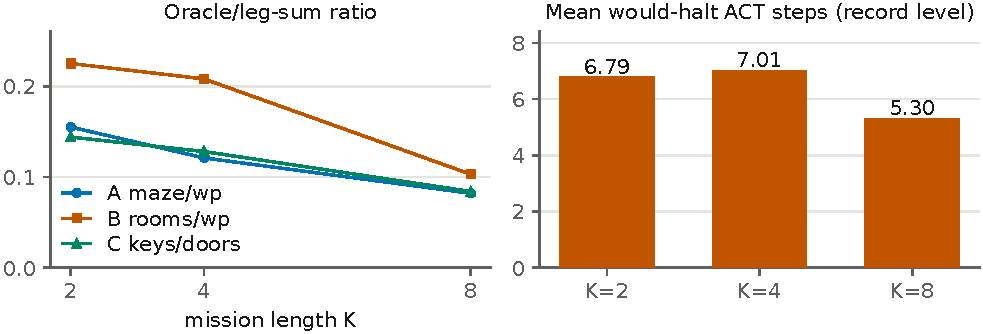
\includegraphics[width=0.98\columnwidth]{figures/fig4_c11.pdf}
\caption{Testing hierarchy under favorable conditions (\stage{C11}). Left: the exact compositional oracle's expansion ratio over a leg-sum baseline \emph{falls} with mission length $K$---headroom for depth-exploiting guidance grows. Right: HRM's learned halting spends \emph{fewer} adaptive-computation steps on deeper missions ($\rho{=}-0.407$ at the record level; $-0.578$, $p{=}5{\times}10^{-5}$ map-clustered)---the opposite of the depth-of-compute hypothesis.}
\label{fig:c11}
\end{figure}

The transfer results above hold across model families: under the matched harness, MLP-style scalar models, ON-LSTMs, HRMs, and U-Nets of comparable complexity all reach similar success on unseen maps, with no consistent winner (the U-Net is often strongest on dynamic suites; the HRM holds the best single-suite ratio; the ON-LSTM dominated the earliest calibrated static stage). Architecture choice, in this regime, is largely free---which is good news for practitioners, and which we probed from three adversarial directions to make sure it is not an artifact.

\textbf{Agnosticism is conditional on the harness.} The same architectures diverge sharply when the harness is wrong: under the scalar objective one collapses to the baseline while another gains $+0.475$ success (\stage{C5}), and on a structured forecasting protocol the ordering \emph{reverses} across tasks (ON-LSTM 0.388 vs.\ HRM 0.265 mean success on one; HRM 71/100 vs.\ LSTM 68--69/100 on another, without uncertainty). Similar-success claims are meaningful only under the controlled conditions of the previous sections.

\textbf{Hierarchy gains no depth dose--response, even when invited to.} We designed a stage \emph{for} hierarchical architectures to win (\stage{C11}): compositional multi-leg missions of length $K\in\{2,4,8\}$ whose exact oracle clears a preregistered headroom gate at 4--12$\times$ over a leg-sum baseline, global map/graph inputs for every arm, six matched architectures, three seeds, 198 checkpoints. Every hierarchy-specific gate came back negative: no structured arm beats the MLP control at two depths with a non-decreasing gap; forcing extra recurrent segments leaves error and expansion curves flat; and learned halting \emph{inverts}---mean would-halt steps are 6.79/7.01/5.30 at $K{=}2/4/8$, an anti-correlation that strengthens under map-clustered reanalysis ($\rho{=}-0.578$, stratified permutation $p{=}5{\times}10^{-5}$; Figure~\ref{fig:c11}). What does appear is an information-structure effect---global-input U-Net/GNN arms beat the MLP at shallow $K$ (ratios $\approx$0.67--0.87; clustered intervals exclude parity in two of three configurations)---and it dissolves by $K\in\{4,8\}$. Five of 33 recurrent cells collapse to constant predictions (a reproducible cap-loss signature; removing padding \emph{worsens} them, revealing pad steps used as free compute), so the worst recurrent cells are optimization pathology, not capacity estimates; a scaled follow-up preserves the ordering (U-Net completion 0.804 vs.\ HRM 0.736 at $K{=}2$, 0.413 vs.\ 0.307 at $K{=}8$, where the scaled HRM exactly matches the leg-sum baseline). Two rescue hypotheses also fail their preregistered gates: a persistent-memory pilot on hidden-regime dynamics closes strongly negative despite proven memory headroom, and an iterative product-graph refiner improves bounded search monotonically with cycles in every cell yet no more at $K{=}8$ than $K{=}2$---while its Bellman residual \emph{worsens}, indicating learned search efficiency rather than value iteration \citep{tamar2016vin,lee2018gppn}.

\textbf{The minimal architecture wins the hardest setting.} The bounded-observation result of the previous section is the sharpest exhibit: the confirmed provider is a small flat MLP, and substituting a trimmed HRM into the identical working method fails its preregistered suite-robustness and path-quality gates (a readout-alignment repair helps transiently at one checkpoint and fails at the endpoint). Granting the recurrent model what per-node application denies it---one genuinely persistent state carried across a query's entire expansion sequence---does not help either: in a preregistered pilot with a matched same-checkpoint reset twin, persistent carry makes frontier ranking \emph{worse} (map-macro MRR delta $-0.029$, 95\% CI $[-0.060,-0.003]$), with post-hoc diagnostics showing long-sequence state growth and score collapse. Independent evidence that drastic simplification preserves this architecture family's benchmark performance \citep{jolicoeur2025trm} points the same way. Our claim stays deliberately bounded---architectures matter at specific regimes, and planner-side hierarchy such as learned subgoals \citep{czechowski2021subgoal} is untouched by these results---but for learned heuristic transfer, complexity bought nothing that the harness had not already determined.

\section{Related Work}

\textbf{Learned heuristics for search.} Bootstrapped heuristic learning \citep{arfaee2011bootstrap}, imitation of clairvoyant oracles \citep{bhardwaj2017sail}, differentiable A\textsuperscript{*} \citep{yonetani2021neuralastar}, transformer grid heuristics \citep{kirilenko2023transpath}, and supervised heuristics for classical planning \citep{ferber2020neural} establish that learned guidance reduces search effort; our contribution is the transfer analysis those results presuppose, and the controlled isolation of the objective/integration conditions the gains ride on. Our focal-ranking result supports, from the integration side, the argument that heuristics should be optimized as rankings rather than cost estimates \citep{chrestien2023rank}. Bounded-suboptimal search supplies the integration vocabulary \citep{pohl1970,pearl1982semiadmissible}; multi-heuristic scheduling \citep{aine2016mha} is a natural extension for unreliable learned signals we did not explore.

\textbf{Dynamic and real-time planning.} Space--time search under moving obstacles follows \citet{silver2005cooperative} and \citet{phillips2011sipp}. The bounded-observation study descends from real-time heuristic search \citep{korf1990rta}, and its inference-time local backup is kin to Real-Time Adaptive A\textsuperscript{*}'s state-local value updates \citep{koenig2006rtaa} and to a single value-iteration module step \citep{tamar2016vin,lee2018gppn}, in the broader spirit of executing the right algorithmic step inside a learned system \citep{velickovic2021nar}.

\textbf{Learning in motion planning.} Learned samplers and end-to-end planners \citep{ichter2018sampling,qureshi2019mpnet} form the complementary tradition on the continuous substrate \citep{kavraki1996prm}; we keep the planner classical and learn only the heuristic, which is what makes frozen cross-environment transfer measurable.

\textbf{Adaptation and architectures.} LoRA \citep{hu2021lora} and weight-space composition \citep{wortsman2022soups,ilharco2022task} frame the few-shot and interpolation findings. The Hierarchical Reasoning Model \citep{wang2025hrm} motivates the architecture audit; independent simplification results \citep{jolicoeur2025trm} align with ours. Evaluation practice follows the reproducibility literature \citep{henderson2018matters,agarwal2021precipice,pineau2021reproducibility}.

\section{Limitations}

Headline results are local single-GPU validations with one primary training seed per stage; stages share trained bases and evaluation maps and are not independent replications. Map-clustered reanalysis covers every quantity this paper quotes, flipping no verdict, but the full-grid refresh of all published tables remains for the camera-ready. The bounded-observation confirmation is one model seed and one cohort; its direct arm carries no formal suboptimality bound (the certified control does), assumes a known roadmap rather than map-free sensing, and its prototype feature construction is slower in wall time than complete-map inference. Dynamic obstacles are deterministic; stochastic motion, kinodynamic constraints, and physical platforms are untested, as is anything beyond 2-D single-agent navigation. All negative findings are failures to observe an effect under the tested protocol, not equivalence claims; in particular, the persistent-state pilot rejects one frozen target/model/training instantiation of planning-time memory, not memory in general.

\section{Conclusion}

Heuristics learned on training maps do transfer to new environments for dynamic path planning---zero-shot with substantial gains, and few-shot along two supervision regimes---provided the training objective and planner integration are right, and largely regardless of model architecture. The practical recipe the analysis supports is short: calibrate the benchmark until the classical baseline can lose; pick the objective that matches the output structure (fields or well-trained scalars, not capped residuals); match the integration to baseline tightness (additive when loose, rank-only when tight); count supervision in labels, not maps, before choosing between low-rank and full adaptation; and spend complexity on none of it---a small model with the right harness transferred further, under less information, than every larger one we trained. The clearest open problems are wall-clock-competitive bounded-observation features, stochastic obstacle motion, and multi-seed replication at scale.

\bibliography{references}

% Check whether the conference requires a reproducibility checklist to be included in the paper.
% If so, you can uncomment the following line and adjust the path to include it.
% \input{ReproducibilityChecklist.tex}

\end{document}
